\documentclass[12pt, a4paper]{article}
\usepackage{graphicx}
\usepackage{pgfplots}
\usepackage{mathtools}
\usepackage{fancyhdr}
\usepackage{multicol}
\usepackage{cancel}
\usepackage{geometry}
\usepackage{listings}
\usepackage{booktabs}
\usepackage{tabularx}
\usepackage{subcaption}
\usepackage[backend=biber,style=apa]{biblatex}
\usepackage{hyperref}
\usepackage{float}
\usepackage{titlesec}
\usepackage{tikz, pgfplots}
\usepackage[utf8]{inputenc}

% Requirement libs
\usetikzlibrary{positioning}

% Options
\nonstopmode % To make sure that you dont have to press input for each error
\geometry{top=1in, left = 1in, right = 1in, bottom=1.2in}
\pgfplotsset{compat=1.18}
\graphicspath{{./figures}}
\setlength{\columnsep}{0.7cm}

% Metadata
\addbibresource{./citations.bib}
\author{Aris Podotas}
\date{\today}

% Herlink setup
\hypersetup{
    colorlinks=true,
    linkcolor=blue,
    filecolor=magenta,
    urlcolor=cyan,
    pdftitle={Project Report MLICB},
    pdfpagemode=FullScreen,
}

% For the code blocks
\definecolor{codegreen}{rgb}{0.03,0.5,0.03}
\definecolor{codegray}{rgb}{0.5,0.5,0.5}
\definecolor{codepurple}{rgb}{0.58,0,0.82}
\definecolor{backcolour}{rgb}{0.95,0.95,0.95}

% Code block setup
\lstdefinestyle{mystyle}{
    backgroundcolor=\color{backcolour},
    commentstyle=\color{codegreen},
    keywordstyle=\color{magenta},
    numberstyle=\tiny\color{codegray},
    stringstyle=\color{codepurple},
    basicstyle=\ttfamily\footnotesize,
    breakatwhitespace=false,
    breaklines=true,
    captionpos=b,
    keepspaces=true,
    numbers=left,
    numbersep=5pt,
    showspaces=false,
    showstringspaces=false,
    showtabs=false,
    tabsize=4,
    escapeinside = {(*}{*)}
}
\lstset{style=mystyle}

% My custom headers and margins 
\pagestyle{fancy}
\setlength{\headheight}{44pt}
\setlength{\headsep}{18pt}
\lhead{\includegraphics[scale = 0.2]{./bnw unit.png}}
\chead{\quad Data Science and Information Technologies Master’s
National and Kapodistrian University of Athens}
\rhead{}
\lfoot{}
\cfoot{\thepage}
\rfoot{}

% Todo: Add citations

% Start
\begin{document}

% Custom title page
    \begin{titlepage}
        \centering
        {\huge \textbf{Final Project}\par}
        \vspace{0.5cm}
        {\Large \textbf{Names:} Aris Podotas, Rafail Adam, George Leventis\par}
        \vspace{0.5cm}
        {\Large \textbf{ID's:} 7115152400040, 7115152400009, 711572100024\par}
        \vspace{0.5cm}
        {\large \textbf{University:} National and Kapodistrian University of Athens\par}
        \vspace{0.5cm}
        {\large \textbf{Program:} Data Science and Information Technologies\par}
        \vspace{0.5cm}
        {\large \textbf{Specialization:} Bioinformatics - Biomedical Data\par}
        \vspace{0.5cm}
        {\large \textbf{Lesson:} Machine Learning in Computational Biology\par}
        \vspace{0.5cm}
        {\large \textbf{Date:} \today \par}
        \tableofcontents
    \end{titlepage}

    \begin{multicols}{2}

        \section{Abstract} \label{sec:Abs}

            In recent years the hematopoietic progenitor cells have been a focal point of research for the key insights to the immune system and cell differentiation they provide. Much of this research has to do with the details of the differentiation of these progenitors to downstream cell types, since this is a key concept that has many intricacies yet to be discovered. Within the reference publication the authors try to deliver some key insights in this process with results that suggest some of the current understanding of this process may be incorrect. Here we hone in on a key issue found in this publication with aim to definitively decide what algorithms should be used in a key step of the pipeline.

        % section Abstract end

        \section{Introduction} \label{sec:Intro}

            \subsection{Overview Of The Publication}\label{sub:Overview Of The Publication} % (fold)

				In recent years, many studies have been focusing on unraveling the differentiation trajectories of the hematopoietic lineage.
                One key aspect of this task is the early differentiation of these cells whose structure sheds light into the origins of each differentiated cell type.
                The challenges that govern this task include the high variability of the human hematopoietic progenitors whose isolation has been mostly based on the marker CD34.
                One caveat that comes from this, is the fact that hematopoietic progenitors are so diverse that some subtypes include cells with lowly expressed CD34 or none at all, which compromises any studies that are solely based on this marker.
                This prompted the authors of this study to use an additional marker , CD164, which they found to be indicative of differentiation according to preliminary data.
                After obtaining two samples, one containing the CD34+ fraction of cells and another the whole bone marrow fraction of cells from two healthy donors, they proceeded with the computational analysis from the single-cell RNA-seq experiment.
                \newline

                Following the filtering out of dying cells, and gene filtering, the expression values were z-scaled and PCA \cite{pearson_lines_1901} was fitted on the sample coming from the whole bone-marrow fraction sample keeping only 40 components and was then used to transform the sample containing only the CD34+ cells.
                A K-nearest-neighbor (KNN) graph was constructed with $k=4$ for every sample and structure aware filtering followed.
                During this step, consolidation points are fitted on the graph whose position is determined by a loss function that changes the structure by using the consolidation points to bring cells closer together within a radius and spread them across the first $2$ Principal components, convergence is achieved if the consolidation points do not move more than a pre-defined threshold.
                \newline

                Branch reconstruction is performed by the use of the minimum spanning tree algorithm and branch association takes place based on the Euclidean distance \cite{ballantine_distance_1952} of each cell from the axis defined by the previous step.
                Finally, the distances between the different branches are measured with the goal of ordering them, giving rise to the final structure.
                \newline

                From these two differentiation structures that are shown, one can clearly observe the diffence in resolution obtained by sampling the whole bone-marrow fraction as well as the finding that the baseophilic branch of cells comes more closely resembles the megakaryocyte progenitors rather than the lymphoid ones

            % subsection Overview Of The Publication (end)

            \subsection{Flaws Of The Paper} \label{sub:Flaws}

            In the methods section of the paper \cite{pellin_comprehensive_2019}, there is mention of one of the initial steps being that of the creation of a K-nearest-neighbor graph (commonly KNN graph). This graph is then mentioned to have been made using a K value $k=4$. No more mention into the reasoning of the value was made, so two key questions arose. One is why the value of $4$ specifically? Considering that odd values are prefers by default. Two is why only the KNN algorithms was used for the generation of the graph with the purpose of partitioning or labeling the cells?
            \newline

            From an otherwise excellently written paper \cite{pellin_comprehensive_2019}, this one methodology choice stuck out.
            \newline

            % subsection Flaws Of The Paper end

            \subsection{Proposals} \label{sub:Prop}

            Our proposals start with the use of a generative model to estimate the gene expression domains for each gene individually across all cell types. This sounds strange since the cell data is available, however after reading the publication carefully there are two available datasets that lead to very different projects. The first dataset is of the cells as they were extracted from the patients. The second is of the results of the analysis in the publication, in a matrix where rows represent unique genes, columns represent groups isolated and values are of gene expression z-scaled. Seeing this, since the second dataset is cleaned (no missing data), pre processed and clear we decided to use that data. Then since we do not have individual cells to cluster as the publication did we would need to generate them using the domain of each gene's expression to estimate and sample expressions. The gene domain was the gene expression along groups (so each row of the matrix). More on the generative model in the methods \ref{sec:Methods} and the results \ref{sec:Res}.
            \newline

            We then proposed alternative methods that can output labels to mitigate the flaws found in section \ref{sub:Flaws}. These methods do not need to use a graph, however some methods that expand on the KNN with more steps were used to try and generate outputs that simply try to better the results of the original graph.
            \newline

            The algorithms chosen:

            \begin{enumerate}
                \item KNN
                \item Single Link
                \item Ward Algorithm
                \item Complete Link
                \item Spectral Clustering
                \item The Chameleon
            \end{enumerate}

            The algorithms are mostly clustering algorithms for the reproduction of the cell labels into groups (clusters).
            \newline

            The reasons elaborated on the relative section \ref{sub:Reasoning}.
            \newline

            % subsection Proposals end

            \subsection{Reasoning}\label{sub:Reasoning} % (fold)

            The choices of the algorithms \ref{sub:Prop} were based on the following few assumptions about the data and the problem at hand.
            \newline

            Assumptions:

            \begin{enumerate}
                \item The clusters are not compact
                \item The data is high in dimensionality
                \item The number of clusters is unknown and expensive to estimate
                \item Clusters form abstract shapes
                \item Cluster bounds will not be clear
                \item There exist rare sub populations of cells
            \end{enumerate}

            The reason the KNN is included is for a direct comparison with the original work. The reason we use the Chameleon and the Spectral Clustering is because they have in initialization using a KNN graph, also the spectral clustering is a subspace clustering algorithm to mitigate the dimensionality of the data. The reason the Single link was chosen is because it outputs elongated clusters and has a graph based approach. The same is true for the Ward and Complete link as far as the graph based approach is involved however they do not output elongated clusters, they were added for reference and to validate this idea of our clusters not being compact.
            \newline

            An added note about one of the assumptions is that since we cannot easily estimate the number of clusters this has removed some algorithms from being viable candidates, so questions of why a specific algorithms was \textit{not} used can be traced to that.
            \newline

            % subsection Reasoning (end)

            \subsection{Limitations}\label{sub:Limitations} % (fold)

            The key limitations are of the generative step, since we estimate the domain of the means over the groups the interpolation between the discreet values will affect the project significantly. To add to this since the generators sample from the distribution based on likely samples, the under represented groups in the data will be hard to generate.
            \newline

            % subsection Limitations (end)

        % section Introduction end

        \section{Methods} \label{sec:Methods}

            Overview of the pipeline.
            \newline

            \end{multicols}

                \begin{figure}[H]
                    \begin{center}
                        \includegraphics[width=0.95\textwidth]{./flowchart.png}
                    \end{center}
                    \caption{Flow chart of the methods done made in \cite{noauthor_excalidraw_nodate}}\label{fig:Flow}
                \end{figure}

            \begin{multicols}{2}

            \subsection{Programming}\label{sub:Programming} % (fold)

                \subsubsection{Dependencies}

                    The project was implemented in Python \cite{noauthor_3132_nodate} using the following libraries:

                    \begin{enumerate}
                        \item numpy \cite{noauthor_numpy_nodate}
                        \item pandas \cite{noauthor_pandas_nodate}
                        \item the chameleon \cite{lin_moonpuckchameleon_cluster_2025}
                        \item sklearn \cite{noauthor_scikit-learn_nodate}
                        \item scipy \cite{noauthor_scipy_nodate}
                        \item matplotlib \cite{noauthor_matplotlib_nodate}
                    \end{enumerate}

                \subsubsection{Implementation Details}

                    The implementations is in multiple files, each for a different part of the results (such as the optimal k search and the optimal algorithms search). Each file contains the same command line input format and it is recommended to read the help menu. Scripts to be directly ran include the knn.py file and the main.py file in the ./src/ directory.
                    \newline

                    Each scrip ran for the generation of the results used $100$ cells and $100$ runs (-cells 100 -runs 100), which is the default for the command line inputs.
                    \newline

                    Keep in mind that the script was made to run on a directory input (-inp) that contains files and will use a listing of the directory (will \textit{not} walk down the directory) to find all files (won't look at extension) to use all DSV (deliminator separated value) files for appending to one, gene $\times$ groups matrix. Also keep in mind that DSV files with multiple sheets will append all sheets to the same matrix. The only file that has the actual gene expression values is "CD34 CD164 GroupLevelExpression" so it was isolated in a separate folder. In this way the recommended way to use the scrip is to isolate the query DSV files into a new folder for each unique run, otherwise the appending of all files will result in non-representative outputs if not just an error.
                    \newline

                    Please note that all runs are written from the perspective of being ran in the ./src/ directory with the current folder structure. The reason is the use of relative paths in the commands however one can use absolute paths as long as they replace all present paths (-inp, -out).
                    \newline

                    Be very careful if you are to use the -clean option of the scripts for it will remove a directory recursively.
                    \newline

                    \textbf{Finding the best K in KNN:}
                    \newline

                    \begin{minipage}{\linewidth}
                    \texttt{python knn.py -out ../knnRun1/ -inp ../data/CDgroup/expression/ \\ CD34\_CD164\_GroupLevelExpression \\ .xlsx}
                    \end{minipage}
                    \newline

                    The output path (after \texttt{-out}) can be any desired output directory.  
                    The input file (after \texttt{-inp}) can have any preceding path to the file.
                    \newline

                    \textbf{Finding the best algorithm:}
                    \newline

                    \begin{minipage}{\linewidth}
                    \texttt{python main.py -out ../testOutput/ -inp ../data/CDgroup/expression/ \\ CD34\_CD164\_GroupLevelExpression \\ .xlsx}
                    \end{minipage}
                    \newline

                    Where the output (after -out) can be wherever you want the output files and the input file (after -inp) could have any preceding path to the file mentioned.
                    \newline

                    Keep in mind that the file paths were not renamed for the \href{https://github.com/ArisPodotas/MLICB-Project}{github repository} and may have a confusing naming scheme. See the default command in case of confusion (from above).
                    \newline

                    Disclaimer: The runs (within script sections aptly named "runs" given by -runs) take around $45$ seconds each, keep in mind that the scrip runs for extended periods of time with the default parameters. Program is overly verbose due to no options being set in one of the dependencies.
                    \newline

                    Source files can be found in the relative \href{https://github.com/ArisPodotas/MLICB-Project}{repository}. Camel case is preferred and functions primarily include documentation strings and type hints. An object oriented approach was followed.

            % subsection Programming (end)

            \subsection{Models and Metrics}\label{sub:Models and Metrics} % (fold)

                As was mentioned in the proposals the Models were:

                \begin{enumerate}
                    \item KNN
                    \item Single Link
                    \item Ward Algorithm
                    \item Complete Link
                    \item Spectral Clustering
                    \item The Chameleon
                \end{enumerate}

                The corresponding metrics were:

                \begin{enumerate}
                    \item Calinski-Harabasz score, also known as the Variance Ratio Criterion \cite{calinski_dendrite_1974}
                    \item Silhouette score \cite{rousseeuw_silhouettes_1987}
                    \item Davies-Bouldin score \cite{davies_cluster_1979}
                \end{enumerate}

                These metrics were used to get a view of the clusters output by a method considering we cannot visualize this high dimensional set even with feature selection. The Calinski-Harabasz score is a measure that will compare the within cluster dispersion to the overall cluster dispersion between clusters, in this way it gives us a view of the clusterings variance with higher values being an indicator of a better fit. The silhouette score will compare how well points from cluster A are described by cluster A as opposed to all other clusters, in this way giving us a measure of how well a fit our clustering is to the data with values ranging from $-1$ to $1$ with higher values being indicative of a better fit. The Davies-Bouldin score is a measure of cluster compactness, in this way it tells us the shape of our clusters with lower values indicating more compactness. Actually our clusters are expected to be arbitrary in shape so the Davies Bouldin score does not necessarily need to be minimized.
                \newline

            % subsection Models and Metrics (end)

            \subsection{Generative Modeling}\label{sub:Generative Modeling} % (fold)

                Five different models were developed for the purpose of generating the new cells from the gene domain distributions. Out of these five only two can be seen as true generative models and the other three were for reference or as a baseline to improve in key directions.
                \newline

                \begin{enumerate}
                    \item Random sampling
                    \item Discreet selection of a pre existing expression
                    \item Gaussian modeling
                    \item Gaussian mixture modeling
                    \item Gaussian Kernel Density Estimates
                \end{enumerate}

                The final results shown here were made using the Gaussian mixture models. Reasons include faster computation time and non discreetized step along any one axis (since the KDE takes small steps to compensate for non continuous functions. It's simply a model fit for another application).
                \newline

            % subsection Generative Modeling (end)

        % section Methods end

        \section{Results and Discussion} \label{sec:Res}

            \subsection{Cell Generator}\label{sub:Cell Generator} % (fold)

                An example of what the generators should estimate:

                \end{multicols}

                    \begin{figure}[H]
                        \begin{center}
                            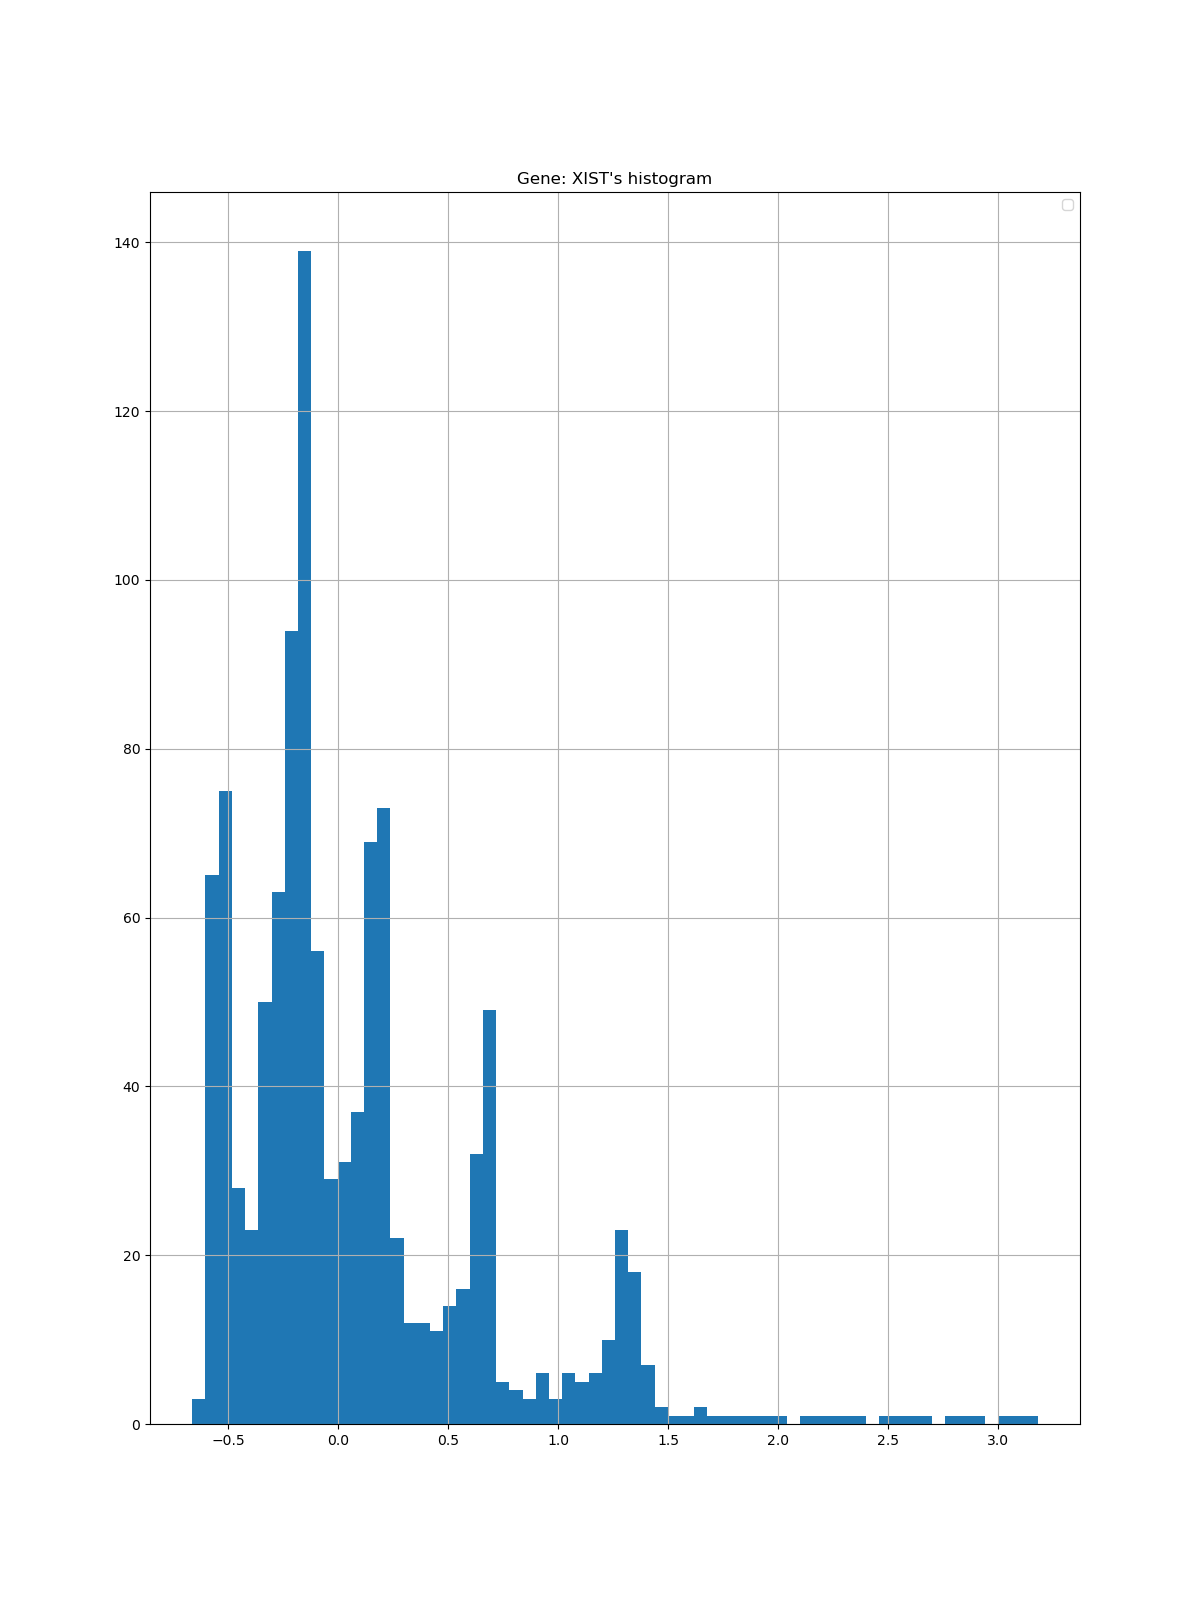
\includegraphics[width=0.95\textwidth]{./outputs/Generator/Histograms/gene_XIST_hist.png}
                        \end{center}
                        \caption{Isolated gene domain (histogram) for a random gene (XIST). The X axis contains values of expression for the gene in question and Y axis values are the frequency of that range of expression in the data.}\label{fig:Dist}
                    \end{figure}

                \begin{multicols}{2}

                Notice that in figure \ref{fig:Dist} the distribution of the gene expression domain is similar to a Gaussian mixture distribution. This is the general form, some genes may look like a standard Gaussian some like other function like $\frac{1}{x}$, some like the figure \ref{fig:Dist} and some other may be discreet in a way that makes it hard to estimate in general.
                \newline

                An example of an output:

                \end{multicols}

                    \begin{figure}[H]
                        \begin{center}
                            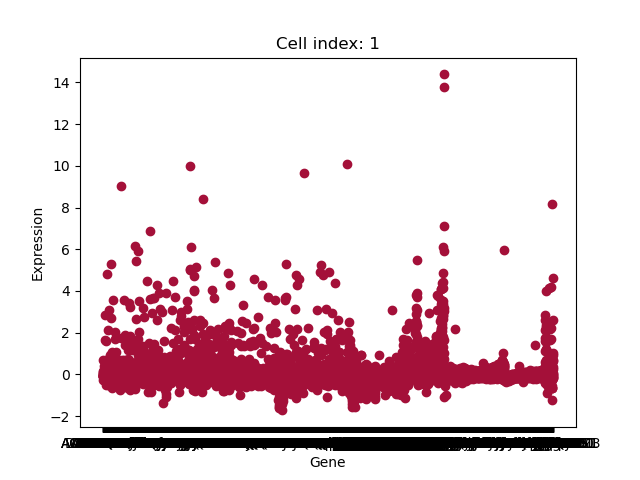
\includegraphics[width=0.95\textwidth]{./outputs/Generator/Cells/Cell 1.png}
                        \end{center}
                        \caption{Visualization of a generated cell. The x axis has the discreet genes, the y the generated expression value. The X axis is of the discreet genes and the Y is of the generated expression value for that gene.}\label{fig:cells}
                    \end{figure}

                \begin{multicols}{2}

                No rigorous way to determine the optimal sampler is done since no metrics exist for this task and thus it was chosen that a Gaussian mixture model should estimate all the distributions used in the analysis as was mentioned in the methods \ref{sec:Methods}.
                \newline

                More figures like figure \ref{fig:Dist} and \ref{fig:cells} can be found in the \href{}{repository}.
                \newline

            % subsection Cell Generator (end)

            \subsection{Optimal K} \label{sub:K}

                It was mentioned in the introduction \ref{sec:Intro} that the KNN graph used in the citation used a K of $4$ with no further explanation. We wanted to test the idea that $k=4$ is the optimal one by running a KNN graph with K values ranging from $3$ to $7$.
                \newline

                \end{multicols}

                    \begin{figure}[H]
                        \begin{center}
                            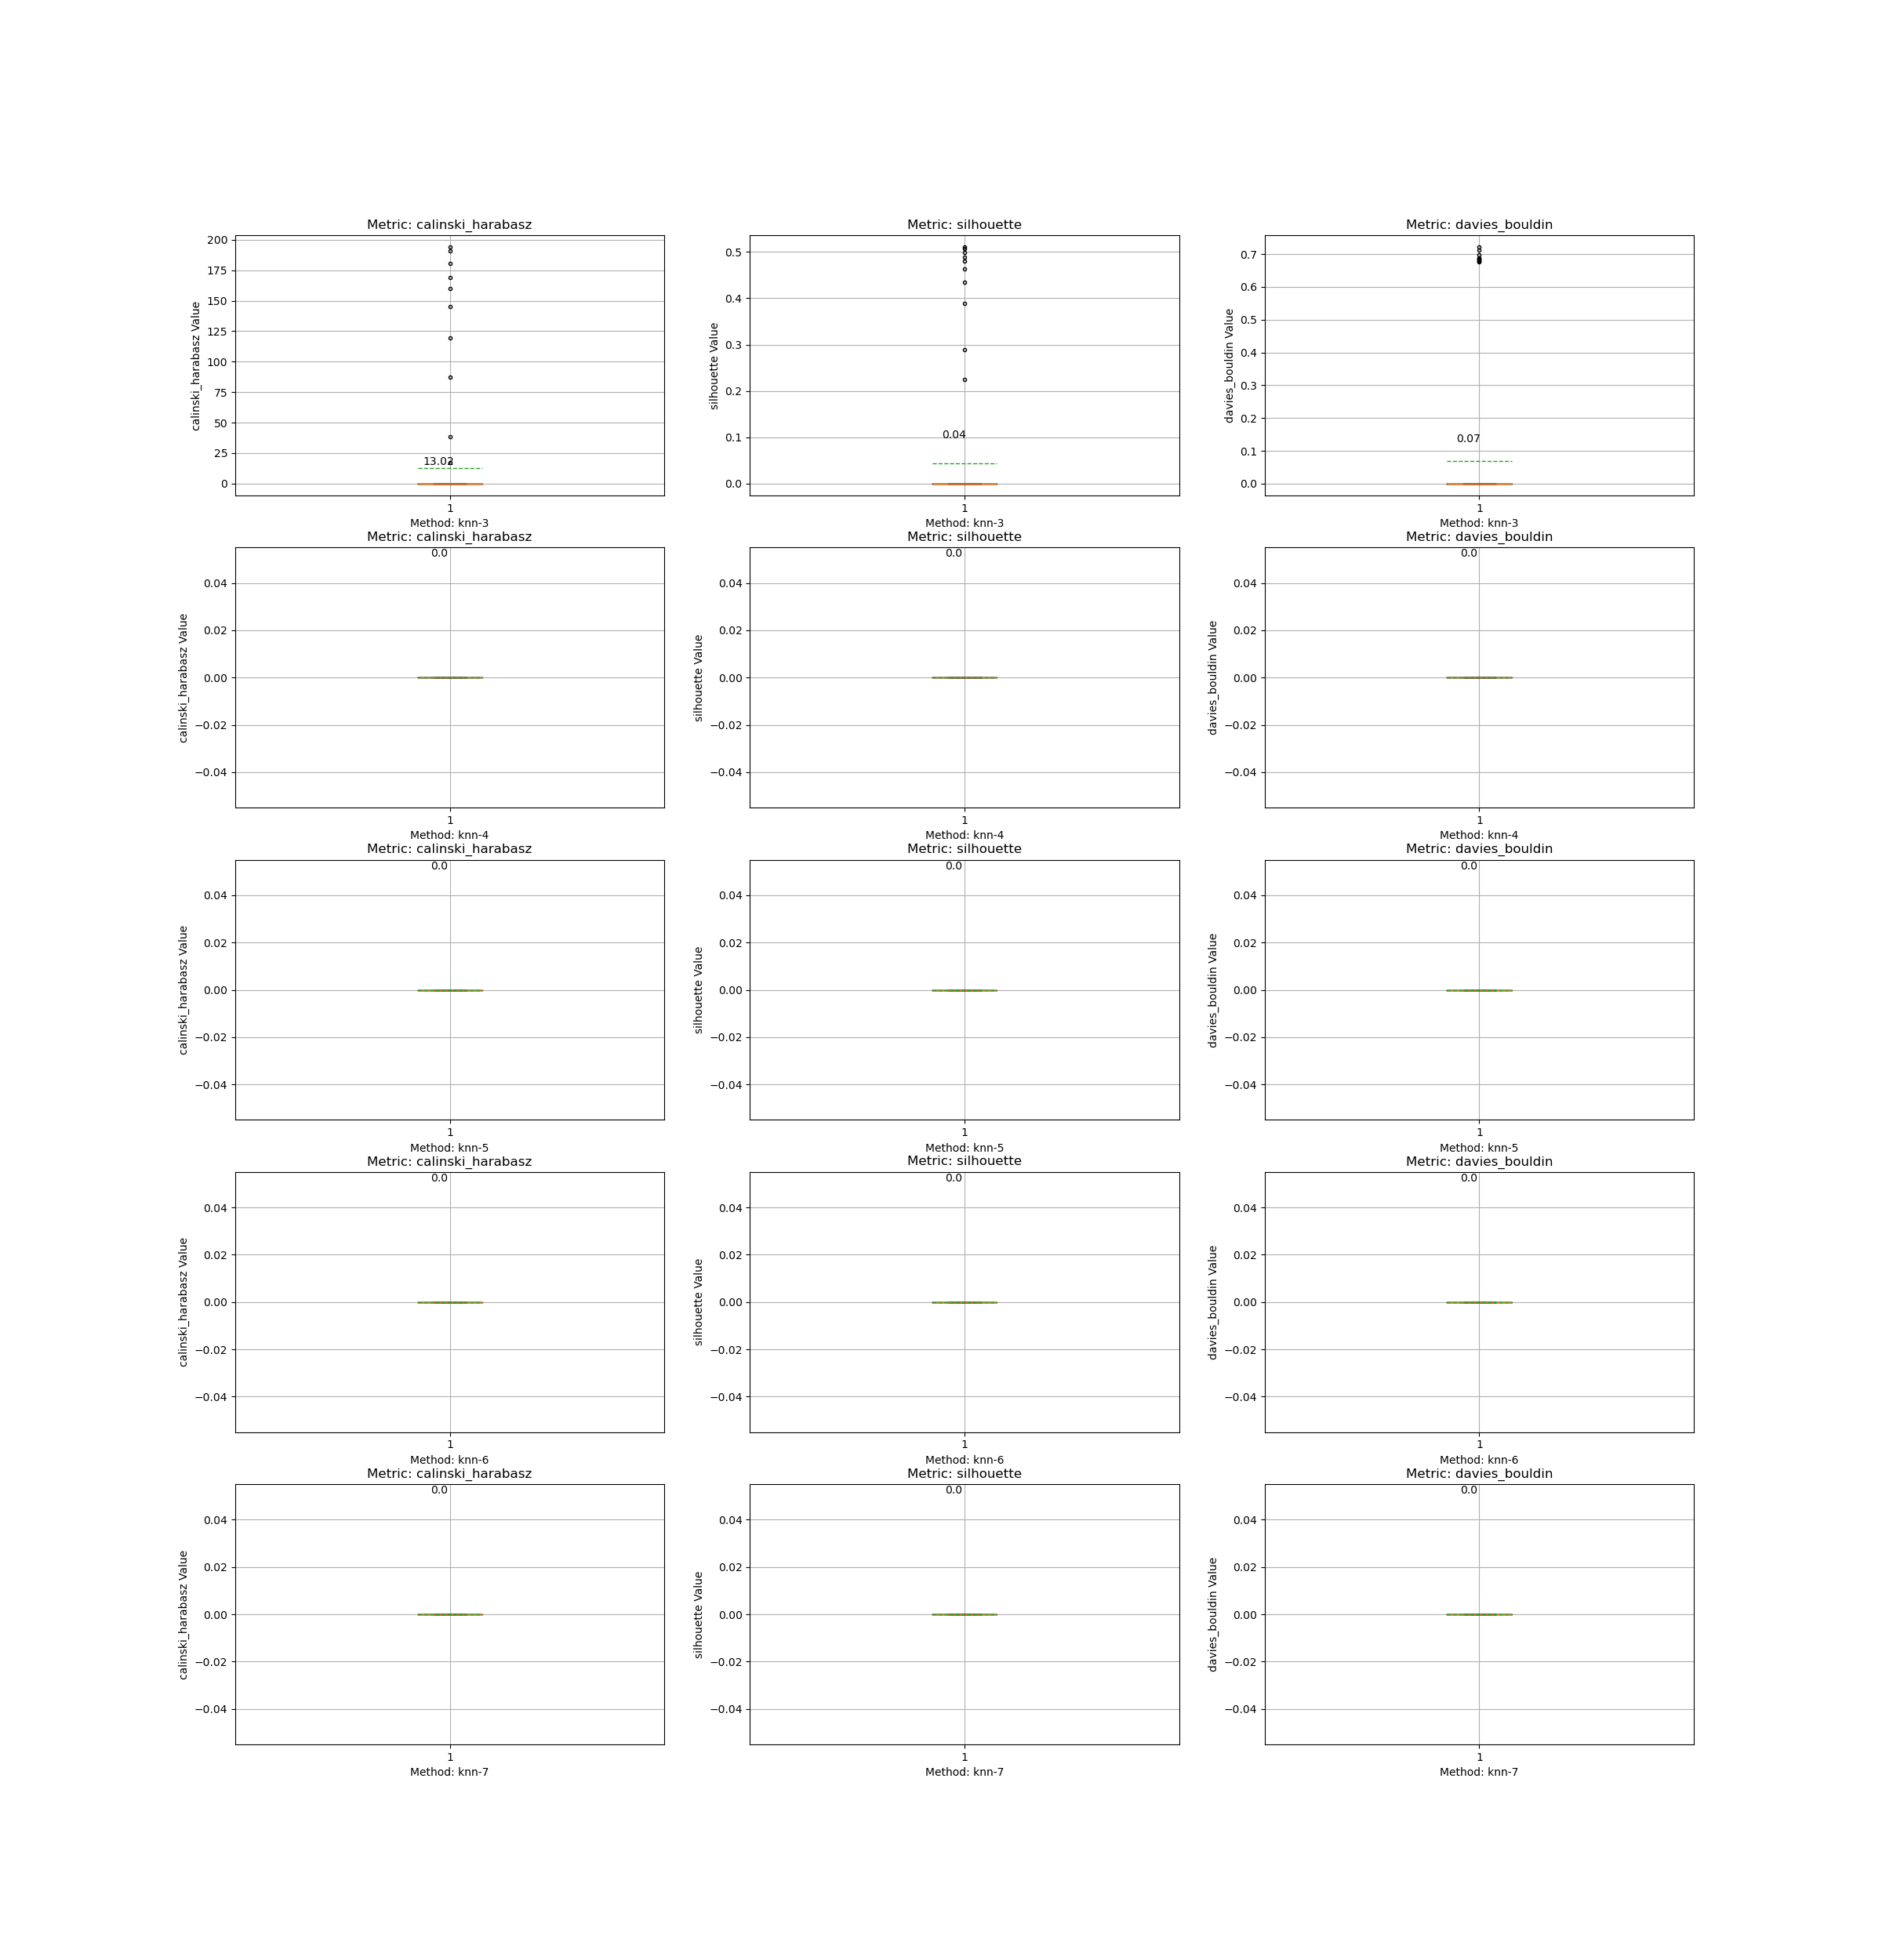
\includegraphics[width=0.95\textwidth]{./knnRun1/full_run_metrics.png}
                        \end{center}
                        \caption{Metrics per KNN run with increasing k. Green dotted lines represent the mean, brown lines represent the median, data labels are of the mean value}\label{fig:Ksearch}
                    \end{figure}

                \begin{multicols}{2}

                It is advised to view images in the original file for greater detail.
                \newline

                One note about the figure \ref{fig:Ksearch} is that the values of K above $3$ are all of a single $0$ value. This is because once a graph unifies the whole data space (cells) into one cluster the metrics all default to $0$. This is actually not as bad as it would seem since for instance the silhouette score ranges from $-1$ to $1$ and the Davies-Bouldin score score is best once lower in value.
                \newline

                It is pretty conclusive that from the figure \ref{fig:Ksearch} that a value of $3$ is optimal for the KNN graph. This would imply that the clusters are fairly close since the value of K is so low and any higher unifies the whole dataset.
                \newline

                In the rest of the assignment (since the k search was the first thing done) the assumed K for any KNN run will be of the optimal K found in \ref{sub:K}.
                \newline

            % subsection Optimal K end

            \subsection{Optimal Algorithm}\label{sub:Optimal Algorithm} % (fold)

                Upon running the algorithms:

                \end{multicols}

                    \begin{figure}[H]
                        \begin{center}
                            \includegraphics[width=0.95\textwidth]{./testOutput/full_run_metrics.png}
                        \end{center}
                        \caption{Metrics per algorithm ran. Green dotted lines represent the mean, brown lines represent the median, data labels are of the mean value}\label{fig:res}
                    \end{figure}

                \begin{multicols}{2}

                It is advised to view images in the original file for greater detail. Keep in mind that the axis is not common before making conclusions.
                \newline

                In figure \ref{fig:res}, we see a few interesting and easy to notice first results. The chameleon has clustered all points to a single cluster and can be seen as generally performing worse than the KNN of $K=3$ and the same as all other K values. The KNN has the most compact output of all algorithms with very low variance distributions (not to be mixed up with variance clustering) and many outliers. The clusters of the KNN are high in variance and the points of one cluster do not fit neatly within one cluster as is evident by the silhouette score.
                \newline

                In figure \ref{fig:res}, the single link has output clusters of not very compact shape as is expected of the algorithm with many outliers evident by the difference between the mean and the median. The points of one cluster do not fit neatly within each cluster as the silhouette score would indicate however with a very high variance. The variance of any one cluster (the variance ratio) is better than the KNN but the worst of the remaining algorithms with a very narrow distribution around the mean value and many outliers.
                \newline

                In figure \ref{fig:res}, the Complete link has done better than all mentioned algorithms thus far in nearly all metrics (depends on how you want to score the Davies-Bouldin score). Metrics are high in variance yet centered around the best mean and median values with considerable differences in the mean and median. Despite the shape of the variance of the metric distribution it would seem that the complete link performs better than the previous two algorithms on it's worst predictor.
                \newline

                In figure \ref{fig:res}, the Ward algorithms narrowly beats out the complete link with very similar distribution in shape. The edges of the distribution reach the same values as the complete link but the mean and median lie just slightly better for all metrics (except the Davies-Bouldin which is just for cluster shape reference). The Ward algorithm is the best performer on this dataset yet.
                \newline

                In figure \ref{fig:res}, the spectral clustering is not too dissimilar to the complete link in the metrics, just slightly better in the variance ration and slightly worse in the silhouette score. The clusters have the most non-compact shape of all algorithms. Let us make a note that in the test the spectral clustering outputs the same as the Ward algorithms but obviously the sampling has had a major effect on the algorithm here.and this is a results that if we had not done as many tests as we have we would not have found. This would suggest that the spectral clustering performs the same as the Ward algorithm in most cell types but there is a subset that differentiates the two algorithms in favor of the Ward algorithm. We overwrote previous results however there is an image the shows this in figure \ref{fig:forSpectral}, the only issue is that the plotting function at the time was not the same and the axis is such that distributions for all metrics are not visible.
                \newline

                In figure \ref{fig:res}, compared to the single link the spectral clustering does have more dispersed distributions of metrics.
                \newline

                \end{multicols}

                    \begin{figure}[H]
                        \begin{center}
                            \includegraphics[width=0.95\textwidth]{./full_run_metrics.png}
                        \end{center}
                        \caption{Metrics per algorithm ran while testing to show the difference of the spectral clustering to the Ward algorithm in other runs. Green dotted lines represent the mean, brown lines represent the median, data labels are of the mean value. Keep in mind that the chameleon had not yet been implemented as this is a old version of the script. This image is for illustrating a point made in the previous paragraph}\label{fig:forSpectral}
                    \end{figure}

                \begin{multicols}{2}

                It is advised to view images in the original file for greater detail.
                \newline

                In figure \ref{fig:forSpectral} we can see that the distribution for at least the variance ratio criterion and the mean values of the rest of the metrics are comparable between the Ward algorithm and the Spectral clustering. This figure is from a version of the script that had a common axis for all plots and thus most metrics are not visible.
                \newline

                Finally, after all consideration it would seem that the Ward algorithms has performed the best of all our proposals based on the metrics.
                \newline

            % subsection Optimal Algorithm (end)

        % section Results end

        \section{Further Research}\label{sec:Further Research} % (fold)
        
            Now that we have the optimal algorithm the original citation should be re visited and if not completely altered to the results of the analysis, should at least contain the multitudes of algorithms and parameter searches. It would improve the methods if the generative model was replaced with real data and if more cells were used to do this analysis. Once iteration with relative results has been completed the following pipeline of the original publication should take place.
            \newline

        % section Further Research (end)

        \section{Supplementary Data}\label{sec:Supplementary Data} % (fold)
        
            \subsection{Reading}\label{sub:Reading} % (fold)
        
                No supplementary text other than this report is needed for understanding the work done.
                \newline

            % subsection Reading (end)

            \subsection{Input Data}\label{sub:Input Data} % (fold)

                Additional files other than the CD34 CD164 GroupLevelExpression file is needed for the analysis however, more input files exist and runs with the whole data were done. Additional data includes every file in the ./Data/ folder that is not CD34 CD164 GroupLevelExpression.
                \newline

            % subsection Input Data (end)

            \subsection{Outputs}\label{sub:Outputs} % (fold)

                Histograms of each gene were made from all supplementary files appended into one structure (as was mentioned in \ref{sec:Methods}) were done and are supplied in the ./outputs/Generator/Histograms/ folder. Keep in mind that these domains include all of the files in the ./Data/ directory from when all of the files were in one single directory without sub directories and to emulate these you would need to make a new folder that has each file within it's top level scope. Keep in mind also that these results of the gene domains were made for proof of concept and are not to be taken seriously since they contain for example gene expressions for the same gene in different individuals and organisms (humand and mice).
                \newline

            % subsection Outputs (end)

        % section Supplementary Data (end)

        \section{Disclaimer}\label{sec:Disclaimer} % (fold)

            Large language models (LLM's) were used during the assignment.

            \subsection{LLM} \label{subsec:llms}

            Open AI: Chat GPT 4.0 \cite{noauthor_chatgpt_nodate}

            \subsection{Purpose} \label{subsec:llmUse}

            \begin{enumerate} \label{enm:llm}
                \item To ask if concepts already exist in some dependency.
                \item For acquisition of the relative documentation.
                \item To validate the idea about the generative model application
                \item To help with the "makeBoxPlots" function
                \item To help convert the graph to labels in the "knn" method of the "ClusterPipeline" class
            \end{enumerate}

        % section Disclaimer (end)

        \printbibliography

    \end{multicols}

\end{document}

